\chapter{Architektura}

BlackBox byl zamýšlen pro tři skupiny uživatelů, přičemž každá má jiné potřeby.
Projekt je rozdělený na tři části, které korespondují se třemi způsoby využití BlackBoxu:

\begin{figure}[h]
    \begin{small}
        \begin{center}
            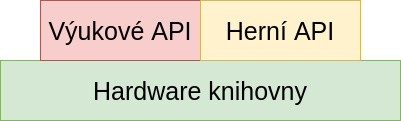
\includegraphics[width=0.95\textwidth]{img/Pyramida2.png}
        \end{center}
        \caption{Tři přístupy}
        \label{fig:Pyramida2}
    \end{small}
\end{figure}

% \begin{enumerate}
%     \item Řídící prvky hardwaru
%     \begin{enumerate}
%         \itema~       
%     \end{enumerate}
%     \item Manager hardware prvků

%     Třída určená pro zjednodušenou práci se všemi prvky hardware naráz, aniž by docházelo ke kolizím.
%     \fxnote{popis co to má být}
% \end{enumerate}

